\documentclass[10pt,twocolumn,letterpaper]{article}

\usepackage{cvpr}
\usepackage{times}
\usepackage{epsfig}
\usepackage{graphicx}
\usepackage{amsmath}
\usepackage{amssymb}

% Include other packages here, before hyperref.
\usepackage{color}
\newcommand{\high}[1]{\scriptsize{\text{\textcolor{red}{#1}}}}
\newcommand{\change}[1]{\textcolor{red}{#1}}

\usepackage{rotating}
% If you comment hyperref and then uncomment it, you should delete
% egpaper.aux before re-running latex.  (Or just hit 'q' on the first latex
% run, let it finish, and you should be clear).
\usepackage[pagebackref=true,breaklinks=false]{hyperref}
%\usepackage{multirow}

 \cvprfinalcopy % *** Uncomment this line for the final submission

\def\cvprPaperID{583} % *** Enter the CVPR Paper ID here
\def\httilde{\mbox{\tt\raisebox{-.5ex}{\symbol{126}}}}

% Pages are numbered in submission mode, and unnumbered in camera-ready
% \ifcvprfinal\pagestyle{empty}\fi
\begin{document}

%%%%%%%%% TITLE
\title{ The Synthesizability of Texture Examples}
\author{Dengxin Dai \quad Hayko Riemenschneider \quad Luc Van Gool\\
Computer Vision Lab, ETH Zurich, Switzerland\\
{\tt\small \{dai, hayko, vangool\}@vision.ee.ethz.ch}
% For a paper whose authors are all at the same institution,
% omit the following lines up until the closing ``}''.
% Additional authors and addresses can be added with ``\and'',
% just like the second author.
% To save space, use either the email address or home page, not both
}

\maketitle
%\thispagestyle{empty}

%%%%%%%%% ABSTRACT
\begin{abstract}
  While example-based texture synthesis~(ETS) has been widely used to
  generate impressive high quality textures of desired size, not all
  images are equally good as the examples.  In this paper we
  investigate the problem of predicting the synthesizability of an
  given image -- how synthesizable it is by ETS.  We introduce a
  database ($21,302$ texture samples) of which all images have been
  annotated in terms of their synthesizability.  We design a set of
  texture features, such as textureness, homogeneity, repetitiveness,
  and irregularity, and train a predictor using these features on the
  data collection.  This work is the first attempt to quantify this
  image property, and we find that synthesizability of images can
  be learned and predicted.  In experiments, we verify the
  effectiveness of several designed features, and verify the
  usefulness of image synthesizability for multiple applications:
  perform an initial selection of examples for large-scale texture
  synthesis, trim images to parts that are more synthesizable, and
  serve as a feature for image recognition.  Also we suggest which
  texture synthesis method is best suited for synthesis of the given
  image.

\end{abstract}

%%%%%%%%% BODY TEXT

\section{Introduction}

\begin{figure} [!t]
  \centering
  \scalebox{0.93}{
   $ \begin{array}{cccc}
\hspace{-1.5mm}
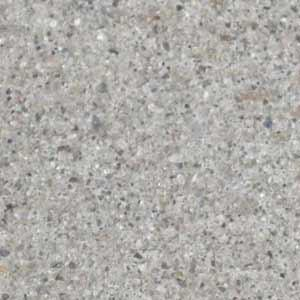
\includegraphics[width=0.33\linewidth]{./figs/fig1/google_concrete_514.jpg} & 
\hspace{-3mm}
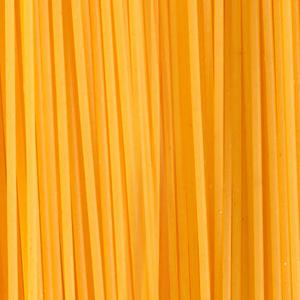
\includegraphics[width=0.33\linewidth]{./figs/fig1/bing2_food_19.jpg}&
\hspace{-3mm}
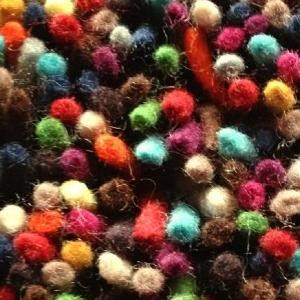
\includegraphics[width=0.33\linewidth]{./figs/fig1/flickr_carpet_300.jpg} \\
\scriptsize{\text{(a) \textcolor{red}{0.99}}} & \scriptsize{\text{(b) \textcolor{red}{0.83}}} & \scriptsize{\text{(c) \textcolor{red}{0.77}}} \\

\hspace{-1.5mm}
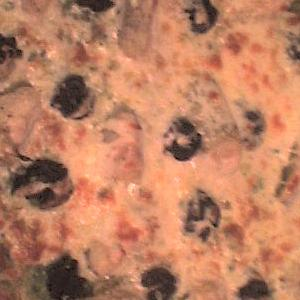
\includegraphics[width=0.33\linewidth]{./figs/fig1/flickr_biscuit_209.jpg} & 
\hspace{-3mm}
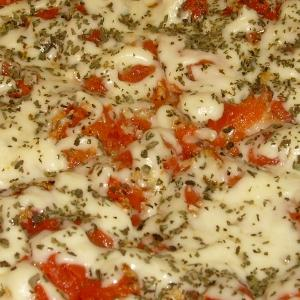
\includegraphics[width=0.33\linewidth]{./figs/fig1/flickr_flour_123.jpg} &
\hspace{-3mm}
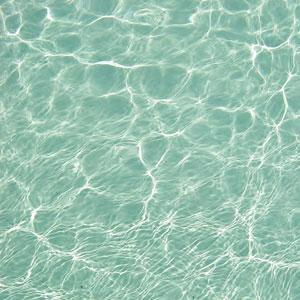
\includegraphics[width=0.33\linewidth]{./figs/fig1/google_water_703.jpg} \\
\scriptsize{\text{(d) \textcolor{red}{0.74}}} & \scriptsize{\text{(e) \textcolor{red}{0.71}}} & \scriptsize{\text{(f) \textcolor{blue}{0.56}}} \\
\hspace{-1.5mm}
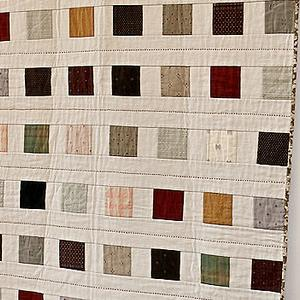
\includegraphics[width=0.33\linewidth]{./figs/fig1/flickr_Fabric_471.jpg} &
\hspace{-3mm}
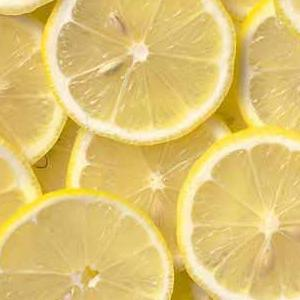
\includegraphics[width=0.33\linewidth]{./figs/fig1/bing2_food_238.jpg} &
\hspace{-3mm}
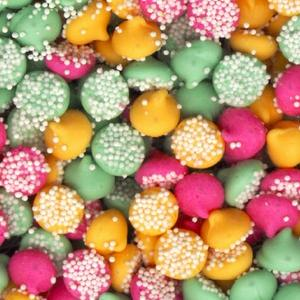
\includegraphics[width=0.33\linewidth]{./figs/fig1/bing2_food_117.jpg} \\
\scriptsize{\text{(g) \textcolor{blue}{0.45}}} & \scriptsize{\text{(h) \textcolor{blue}{0.40}}} & \scriptsize{\text{(i) \textcolor{blue}{0.37}}} \\
\hspace{-1.5mm}
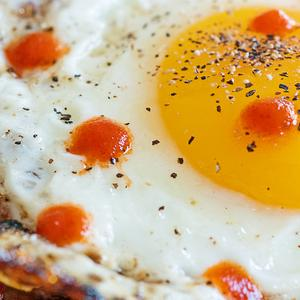
\includegraphics[width=0.33\linewidth]{./figs/fig1/flickr_chips_144.jpg} & 
\hspace{-3mm}
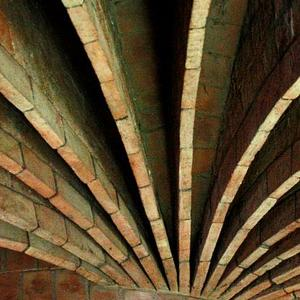
\includegraphics[width=0.33\linewidth, height=27.5mm]{./figs/fig1/flickr_brick_215.jpg}&
\hspace{-3mm}
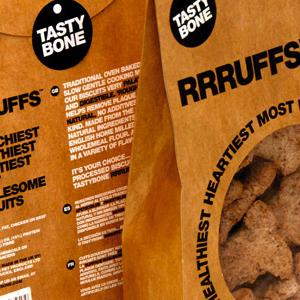
\includegraphics[width=0.33\linewidth]{./figs/fig1/bing2_food_75.jpg} \\
\scriptsize{\text{(j) \textcolor{blue}{0.30}}} & \scriptsize{\text{(k) \textcolor{blue}{0.19}}} & \scriptsize{\text{(l) \textcolor{blue}{0.13}}} \\

\end{array}$}
\caption{Synthesizability of texture examples detected by
  our system. All images are of $300\times 300$ pixels.}
  \label{fig:synlity}
\end{figure}


%% ABILITY TO MEASURE synthesizability
A substantial amount of work has been devoted to synthesising textures
from examples~\cite{Heeger:95,
  Portilla:2000:IJCV,Efros:sig2001,Kwatra:2003, Lefebvre:2005:sig,
  Ma:2011,dai:facade:iccv13}. We will refer to such example-based
texture synthesis as `ETS' in the remainder of this paper. Even if the
set of textures that can be successfully synthesised that way has
steadily been growing, it is often not clear beforehand whether ETS
would be successful for a specific texture sample. It would be
interesting if we were able to predict its synthesizability -- how
well its underlying visual patterns can be re-synthesized by learning
only from the sample. Even if challenging, the task may be doable,
given that other qualitative image characteristics could be
quantified, like quality~\cite{image:quality},
memorability~\cite{image:memorability}, or
interestingness~\cite{image:interestingness}.


%% PROBLEM WITH TEXTURES IN THE WILD
While ETS has proven to be a powerful tool to generate large-scale textures~\cite{WLKT09},
providing texture examples is not straightforward~\cite{lockerman2013arxiv}. ETS systems
typically expect a rectangular sample image, representing a head-on
view of a flat, outlier-free textured surface. Not just any example
image returned by an image searching engine (by typing keywords) will
do.  Such retrieved images may contain outliers, cluttered
backgrounds, distorted texture surfaces, or even objects and other
texture categories. Being able to rank retrieved images in terms of
their synthesizability can then at least perform an initial
selection. It can also be used to trim images to regions with good
synthesizability, by e.g.~removing undesirable
background. Furthermore, synthesizability can help select an
appropriate ETS method. The optimal approach -- also taking into
account speed and stability -- will depend on the texture
and the application. Quilting~\cite{Efros:sig2001} is very potent, for instance, but will
tend to produce verbatim repetitions that become salient when larger
areas need to be synthesized. It would be good if in such case one
could take recourse to an alternative method that does not produce
such issues. Last but not least, studying synthesizability as a
general image property is also an interesting problem.

Fig.~\ref{fig:synlity} shows the synthesizability scores assigned to some texture samples 
by our system. Fig.~\ref{fig:roi} illustrates the trimming of an image to its most
synthesizable, rectangular regions (the red cut-outs).

In order to learn image synthesizability and evaluate its performance, we have collected
a fairly large texture database of $21,302$ texture images. This database has been manually annotated 
in terms of the synthesizability of each image. The synthesizability is characterised as the 
`goodness' of the `best' synthesized texture by a set of ETS methods. The `goodness' is quantified 
as one of three levels: good, acceptable, and bad. See Fig.~\ref{fig:dataset} for examples. 

% {\bf IT IS NOT CLEAR WHAT KIND OF ANNOTATIONS
% THESE ARE: MANUALLY DONE… OR THE SCORES AUTOMATICALLY GIVEN BY OUR METHOD? IF MANUALLY
% DONE, IT IS NOT CLEAR HOW TO COME UP WITH NUMBERS AS IN FIG.1, SO FAR THE GOOD-ACCEPTABLE-BAD 

% CLASSIFICATION HAS NOT BEEN INTRODUCED.}

As to the automated synthesizability scoring, a series of features that would seem to be connected with the task are defined.
A scoring function is then learned from the collection of annotated data.
The experimental results show that automated synthesizability scoring is quite possible.
We also show in experiments that image synthesizability is also helpful for image recognition.

Our main contribution are: (1) to learn the image property
synthesizability methodologically; (2) to design several novel
features for qualitative texture analysis (esp. textureness,
homogeneity, repetitiveness, and irregularity); (3) to offer a fairly
large texture dataset together with synthesizability annotations; (4)
to verify the usefulness of synthesizability in multiple vision
applications.


The remainder of the paper is organized as follows.
Sec.~\ref{sec:related} reports related work.
Sec.~\ref{sec:data} is devoted to our dataset, followed by our features and learning method in Sec.~\ref{sec:feature}.
Sec.~\ref{sec:experiment} presents our experiments and Sec.~\ref{sec:conclusion} concludes. 


\section{Related work}
\label{sec:related}

\textbf{Example-based texture synthesis.}  Techniques of example-based
texture synthesis can be broadly categorized into four categories:
feature-oriented image synthesis~\cite{Heeger:95, Debonet:97,
  Portilla:2000:IJCV, random:phase}, Markov Random Fields (MRFs)
methods~\cite{paget:tip98, zhu:frame, Zalesny05}, neighborhood-based
methods~\cite{Efros:sig2001, Kwatra:2003, Kwatra:tog:2005,
  dai:facade:iccv13}, and tile-based methods~\cite{Cohen:2003:wang,
  Liu:2004:NTA}.  The first group learns statistics of a brand of
carefully designed features and coerces the synthetic images to
have/achieve similar values, e.g. color histograms~\cite{Heeger:95},
multi-band spacial frequencies~\cite{Debonet:97}, and wavelet
features~\cite{Portilla:2000:IJCV}. This group of methods are stable
and do not generate verbatim repetition, but the main challenge lies
in designing a common set of features that is able to capture the
essence of all kinds of textures.  The second group considers textures
as instances of MRFs. Parameters of some forms of MRFs are estimated
from the texture examples and new textures are then sampled from the
model. Multi-scale neighborhood-based MRFs are learned
in~\cite{paget:tip98} and pairwise clique-based MRFs
in~\cite{Zalesny05}. This stream of methods have solid theories, but
are computationally expensive. The third group generate textures by
copying pixels or patches from the exemplar inputs~\cite{Efros:1999,
  Efros:sig2001, Kwatra:2003, Kwatra:tog:2005,
  dai:facade:iccv13}. Unlike the first two groups they do not provide
cues for texture analysis, but this group are often more efficient and
tend to work for a larger variety of textures. The last group assemble
new textures out of a set of (rectangular) tiles cropped from example
images. This stream of methods are very efficient once the tiles are
estimated. However, identifying these tiles is non-trivial:
\cite{liu:ijcv:05} handled this problem by estimating the translation
symmetries, and \cite{dai:facade:iccv13} by detecting the semantic
labels.

\textbf{Texture recognition.}  Our work is also related -- albeit
rather weakly -- to material recognition that also represents a
texture characterization task. Features have been designed to
recognize textures from different material categories, including
statistics of filter responses~\cite{texton:2001, Manjunath96,
  Schmid01}, joint intensity distributions within a compact
neighborhood ~\cite{material:pami:09, sorted:texture}, geometric
features over topographic maps~\cite{xia:texture}, and high-level
semantic attributes~\cite{semantic:texture, texture:wild}.  Similarly,
we need to design appropriate features for this new task.


%%%%%%%%%%%%%%%%%%%%%%%%%%%%%%%%%%%%%%%%%%%%%%%%%%%%%%%%%%%%%%%%%%%%%%%%%%

\section{Data collection}
\label{sec:data}
Although one may have the intuition that the texture patterns of some
images are easier to be re-synthesized than those of other images,
quantifying this intuition has not been addressed. In order to learn
image synthesizability, we collected a database and annotated it in
terms of synthesizability. $40,000$ images were downloaded from
Google, Bing, and Flickr by providing $60$ keywords. The keywords used are
to cover common material classes such as glass, water, stone, plastic,
fabric, leather, metal and paper, and to cover common geometric
texture properties such as stochastic, repetitive, lined, speckled,
wrinkled and cracked. All images were truncated to $300 \times 300$
pixels, with images smaller than this not being used. Since the
retrieved images are very `noisy': a lot of images are not textures,
or they are severely watermarked, we made a manual selection for the
truncated images. Finally, we end up with a dataset of $21,302$
texture samples. 

For the annotation, we characterize the synthesizability of a texture
as the goodness of the best synthesized image generated by a selected
set of ETS methods. A good synthesized image should be as similar as
possible to the input example and should not have visible artefacts
such as seams, blocks and misfitting edges, and should not contain
salient repetitions of sub-patterns in a verbatim fashion, if that is
not the case in the original. Since no ETS method performs better than
all others on all kinds of textures, the annotator got the
choice between the results of four specific methods, that are based on
different methodologies: an image quilting
method~\cite{Efros:sig2001}, a multi-scale Markove Random Field (MMRF)
method~\cite{Zalesny05}, a wavelet-based parametric
method~\cite{Portilla:2000:IJCV}, and a random phase
synthesis~\cite{random:phase}. While future work will probably yield
more powerful ETS methods still, this dataset constitutes an initial
benchmark, based on the current state-of-the-art in ETS. The final
outcome of the annotation for a texture example is the `goodness' of
the synthesized result (among the 4) that the annotator considers
best. This goodness is expressed a one of 3 levels: good, acceptable,
and bad, assigned synthesizability scores of $1$, $0.5$ and $0$,
resp..  The `best' method of each texture example was also recorded to
learn which method is the best to synthesize a given texture example.
In total, we had $25.5\%$ samples labeled bad, $39.7\%$ acceptable and
$34.8\%$ good.  Fig.~\ref{fig:dataset} shows examples of such
annotation.  

%The dataset (incl. images and synthesizability
%scores) is publicly available at the project page.

\begin{figure} [!t]
  \centering
   $ \begin{array}{cccc}
\hspace{-1.5mm}
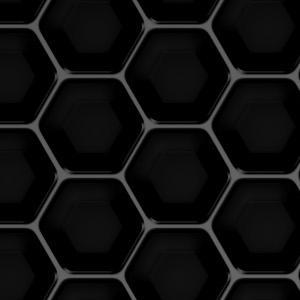
\includegraphics[width=0.23\linewidth]{./figs/dataset/87.jpg} & 
\hspace{-3mm}
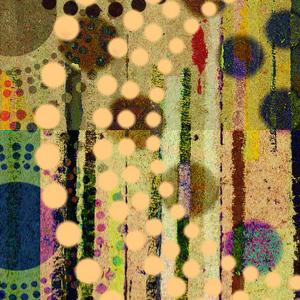
\includegraphics[width=0.23\linewidth]{./figs/dataset/flickr_cardboard_102.jpg} & 
\hspace{-3mm}
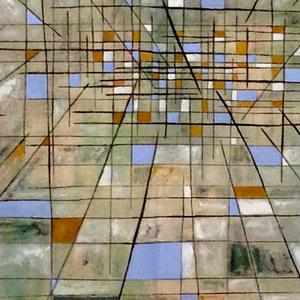
\includegraphics[width=0.23\linewidth]{./figs/dataset/flickr_canvas_358.jpg} \\ 
% \hspace{-1.5mm}
% 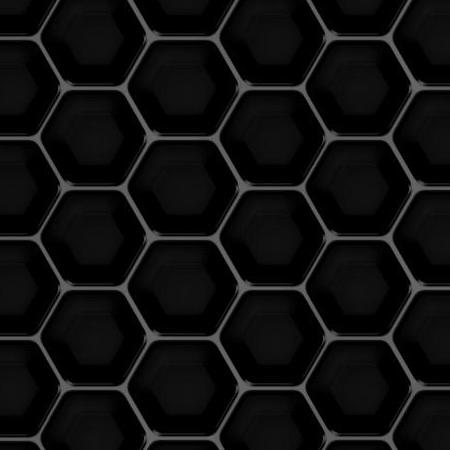
\includegraphics[width=0.33\linewidth]{./figs/dataset/87syn.jpg} & 
% \hspace{-3mm}
% 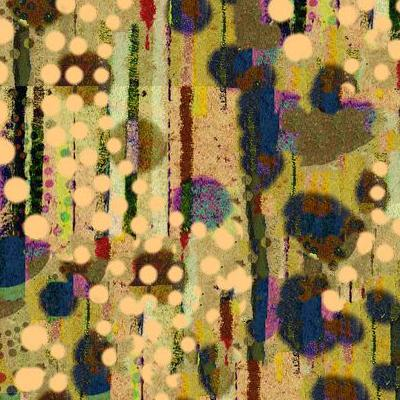
\includegraphics[width=0.33\linewidth]{./figs/dataset/flickr_cardboard_102_q.jpg} & 
% \hspace{-3mm}
% 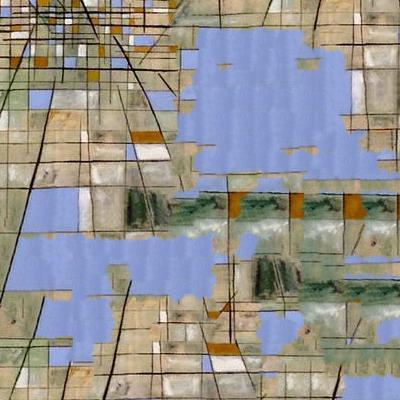
\includegraphics[width=0.33\linewidth]{./figs/dataset/flickr_canvas_358_q.jpg} \\ 
\scriptsize{\text{(a) good:1}} & \scriptsize{\text{(b) acceptable:0.5}} & \scriptsize{\text{(c) bad:0}}  \\

\end{array}$
\caption{Three texture examples from our dataset with their
  annotations of synthesizability, where top are texture exemplars and
  bottom corresponding synthesized textures. }
  \label{fig:dataset}
\end{figure}


%%%%%%%%%%%%%%%%%%%%%%%%%%%%%%%%%%%%%%%%%%%%%%%%%%%%%%%%%%%%%%%%%%%%%%%%%

\section{Learning image synthesizability} 
\label{sec:feature}
In this section, we investigate the visual features relevant to 
image synthesizability. We start from general image features, to move
on to our designed texture features, and to the learning method.

%=======================================================================

\subsection{General features}

% \textbf{Wavelets}. Wavelets have been widely used for texture
% analysis, so we allowed them to contribute to image synthesizability. 
% The complex pyramid wavelet transform on $4$ pyramid levels, with 
% sp3Filters, was used, due to its promising performance on texture 
% analysis/synthesis~\cite{Portilla:2000:IJCV}.

\textbf{Local patterns}. Local binary patterns (LBP)~\cite{lbp:2002}
has been widely used in texture recognition and features of the same
kind achieved s-o-a classification performance~\cite{sorted:texture}. Thus, 
we include LBP as one of our feature, where  uniform LBP is adopted.

\textbf{Filter responses}. Using image filters has become one of the
most popular tools for texture analysis~\cite{texton:2001, Manjunath96}
and synthesis~\cite{zhu:frame}. Thus, we believe that filter responses
are also helpful for learning synthesizability. The Schmid Filter
Bank~\cite{Schmid01} is employed with 13 rotationally invariant
filters at multiple scales.

\textbf{GIST feature}.  Frequency analysis has proven  very useful for
texture analysis/synthesis~\cite{vangool:83, Manjunath96, Debonet:97}, so features of this kind 
should also be used for learning synthesizability.
GIST feature~\cite{gist} is used, where the 
implementation resizes images to $256 \times 256$ pixels, uses only
one grid, and produces a feature vector of dimension $20$.

% \textbf{Self-similarity}. Sufficiently small patches of textures are 
% self-similar in appearance. Thus, it is interesting to evaluate the 
% self-similarity feature~\cite{self:similarity}. We averaged the 
% self-similarity
% vectors of all pixels in an image to represent its self-similarity.

% \textbf{Complexity}. We follow~\cite{image:interestingness} to measure
% the complexity of an image by comparing its JPEG compressed size
% against its uncompressed size. The lower the compression rate, the 
% more complex the texture pattern is. This measure is interesting as
% JPEG has been conceived with human image perception in mind. 

% \textbf{Colorfulness}. The complexity of a texture is also reflected 
% by its colorfulness: the more colors are
% involved in the texture patterns, the more complex the textures tend
% to be. We measure colorfulness as proposed by Datta and Wang~\cite{aesthetic:eccv06}, \ie
% the Earth Mover distance of the color histogram of the texture image
% to a uniform color histogram (representing the most colorful image).
% The smaller the distance, the more colorful (complex) the texture.

% \textbf{Edge length}. It is observed that examples with long edges are
% harder to synthesize than those with shorter edges. A histogram of the
% length of edges is used to characterize this property. We use the
% Canny edge detector~\cite{canny:edge} for edge detection, with the
% high and low thresholds put to $0.6$ and $0.24$, resp.  The histogram
% of $8$ bins is used with the following separating positions: $2, 5,
% 10, 20, 50, 100, 200$.


% SHAPE PRIMITIVES
% \textbf{Shape primitives}.  Apart from generic edges, we further
% investigate the presence of basic shape primitives.  Straight lines
% and corners may be easier to reproduce than complex, irregular shapes.
% For this purpose, we extract local edge fragments with the Canny
% edges.  These local fragments are described by a `self-embedded local
% shape descriptor'~\cite{hayko:eccv2010} which captures the local shape
% by dense angular representation.  We train a vocabulary of shape
% fragments by clustering on the Brodatz texture datasets.  A histogram
% over these shape fragments is then used to describe the presence of
% local shape primitives.


% \textbf{Entropy}.  To capture the complexity of an image, image
% entropy is also measured. Entropy is a statistical measure of
% randomness that can be used to characterize the texture of the input
% image.

% \textbf{structures} cf.~\cite{tsmoothing2012}: texture and main
% structure exhibit completely different properties, makign them
% surprisingly decomposable. We do not assume specific regularity and
% symmetry of the texture patterns: non-uniform and anistropic texture,
% can be handled in a unified framework.
% We do not assume or manually determine the type of textures, as the
% patterns could vary a lot in different examples. 

% Relative Total Variation (RTV) is simple and yet very effective to
% make main structures stand out, thanks to the characteristics of $D$
% and $\phi$.

% \textbf{Patch PCA}.  The randomness of a texture is signaled by the
% intrinsic dimensionality of local texture patches.
% Patches from random textures normally have a higher intrinsic
% dimensionality than patches from smooth textures. Therefore, we
% perform principal component analysis on local patches sampled from the
% texture image and use their intrinsic dimensionality as a feature.
% Specifically, we sampled patches of $20\times 20$ pixels, centered at
% every pixels of the image, and searched for the dimensionality that
% keeps $85\%$ of the energy. This intrinsic dimensionality normalized 
% by the original dimensionality of the patches, i.e. $400$, is used. 

%This feature has been used
%already for image quality prediction~\cite{blind:quality:cvpr11}.

% Textureness

\subsection{Designed features}

\begin{figure} [!t]
  \centering
\scalebox{0.94}{
   $ \begin{array}{cccc}
\hspace{-1.5mm}
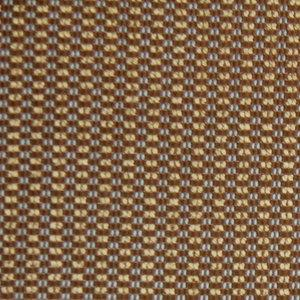
\includegraphics[width=0.33\linewidth]{./figs/repet/1.jpg} & 
\hspace{-3mm}
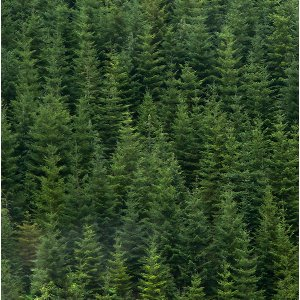
\includegraphics[width=0.33\linewidth]{./figs/repet/forest.jpg} & 
\hspace{-3mm}
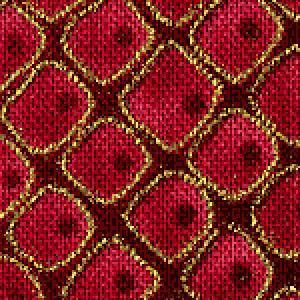
\includegraphics[width=0.33\linewidth]{./figs/repet/352.jpg} \\ 
\scriptsize{\text{(a) 70.25}} & \scriptsize{\text{(b) 21.85}} & \scriptsize{\text{(c) 13.69}}  \\
\hspace{-1.5mm}
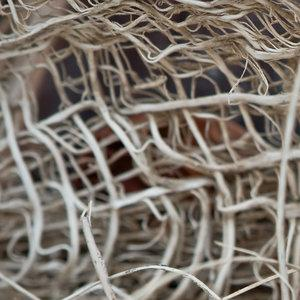
\includegraphics[width=0.33\linewidth]{./figs/repet/439.jpg} & 
\hspace{-3mm}
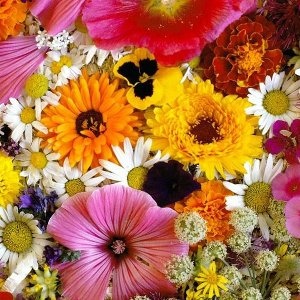
\includegraphics[width=0.33\linewidth]{./figs/repet/flower2.jpg} & 
\hspace{-3mm}
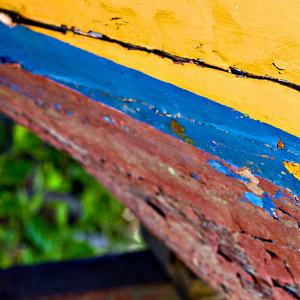
\includegraphics[width=0.33\linewidth]{./figs/repet/832.jpg} \\ 
\scriptsize{\text{(d) 9.04}} & 
\scriptsize{\text{(e) 3.22}} & 
\scriptsize{\text{(f) 2.06}}  \\

\end{array}$}
\caption{The homogeneity of texture examples detected by our
  method. Images are all of $300 \times 300$ pixels.}
  \label{fig:homo}
\end{figure}

% \textbf{Edge coverage}.  
% \textbf{Attributes} lined or circled~\cite{semantic:texture}? 

\textbf{Textureness}. Objects and scenes are more difficulty to
synthesize than textures.  We train a classifier to distinguish
textures from objects and scenes. The UIUC texture
dataset~\cite{UIUC:Texture} delivered the positive samples (textures),
and the 15-Scene dataset~\cite{lazebnik:cvpr06} the negative ones
(objects/scenes). Linear SVMs were used with GIST~\cite{gist} as the
feature. The classification score is taken as textureness.

% Homogeneity
\textbf{Homogeneity}. Homogeneous textures are easier to be
re-synthesized than heterogeneous ones.  Thus, it is desired to have a
feature measuring the homogeneity of images. One that has been
proposed is based on co-occurrence matrices~\cite{texture:analysis},
which is very low-level and sensitive to noise. We here propose a
simple, yet more robust method.

\noindent 
\textbf{Definition:} The homogeneity of an image is the expectation of
visual similarity between two randomly-chosen local regions of the image.

In particular, given an image
$X \in \mathbb{R}^{H\times W}$, we measure the averaged similarity over $T$ trials. 
In trial $t$, two regions $R_1^t$
and $R_2^t$ are sampled from $X$, and their distance
$d(R_1^t, R_2^t)$ is measured. The homogeneity of $X$ is then:
\begin{equation}
  \label{eq:repet}
\text{Hom}(X) = \frac{1}{T}\sum_{t=1}^T \frac{1}{d(R_1^t, R_2^t)}.  
\end{equation}
$R_1^t$ and $R_2^t$ are of the same size $\lfloor H/3 \rfloor \times \lfloor W/3 \rfloor$, and their
positions are sampled uniformly, at random from $\{(i,j): i\in\{1,
..., \lfloor 2H/3 \rfloor \}, j\in \{1, ..., \lfloor 2W/3 \rfloor \} \}$. Images (regions) are
represented with bag-of-words. The dictionary is learned from $X$ by
k-means with $30$ centres on patches of size $10\times 10$ cantered at
every pixel (RGB values are used). See Fig.~\ref{fig:homo} 
for the homogeneity of six texture examples detected by the method.
Our homogeneity is more effective than the co-occurrence matrices one ~\cite{texture:analysis} because 
the measurement is performed on typical visual parts instead of pixel intensities, 
and more robust because the histogram of regions introduces local spatial invariance. 
 
%  \textbf{low-rank texture} 
% Our intuitive distinction between these two kinds
% of data is that textur
% ~\cite{low:rank:texture:ijcv12}. 

\begin{figure} [!t]
  \centering \scalebox{0.94}{
   $ \begin{array}{cccc}
\hspace{-1.5mm}
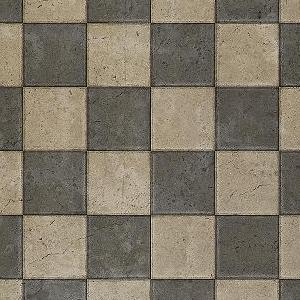
\includegraphics[width=0.33\linewidth]{./figs/repetitiveness/bing2_floor_201.jpg} & 
\hspace{-3mm} 
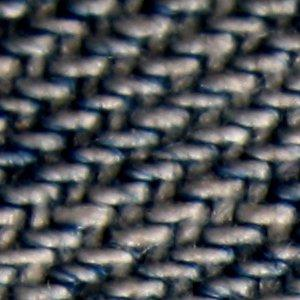
\includegraphics[width=0.33\linewidth]{./figs/repetitiveness/60.jpg} & 
\hspace{-3mm}
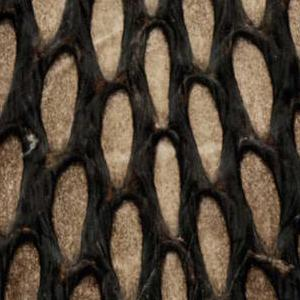
\includegraphics[width=0.33\linewidth]{./figs/repetitiveness/bing2_animal_19.jpg} \\ 
\scriptsize{\text{(a) 2.44}} &
 \scriptsize{\text{(b) 2.04}} & 
\scriptsize{\text{(c) 1.93}}  \\
\hspace{-1.5mm}
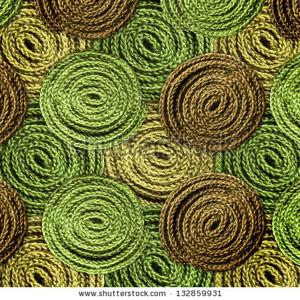
\includegraphics[width=0.33\linewidth]{./figs/repetitiveness/13rep.jpg} & 
\hspace{-3mm}
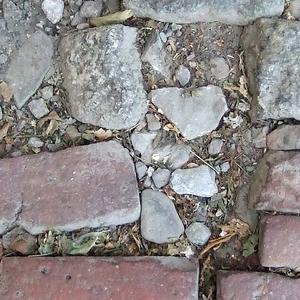
\includegraphics[width=0.33\linewidth]{./figs/repetitiveness/flickr_crushed_58.jpg} & 
\hspace{-3mm}
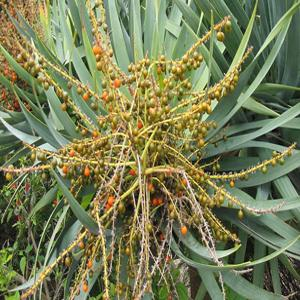
\includegraphics[width=0.33\linewidth]{./figs/repetitiveness/9rep.jpg} \\ 
\scriptsize{\text{(d) 1.43}} & 
\scriptsize{\text{(e) 1.39}} & 
\scriptsize{\text{(f) 1.38}}  \\
\hspace{-1.5mm}
\includegraphics[width=0.33\linewidth]{./figs/repetitiveness/cv/cv_60.jpg} & 
\hspace{-3mm}
\includegraphics[width=0.33\linewidth]{./figs/repetitiveness/cv/cv_2.jpg} & 
\hspace{-3mm}
\includegraphics[width=0.33\linewidth]{./figs/repetitiveness/cv/cv_9rep.jpg} \\ 
\scriptsize{\text{(g): NCC map of (a)}} & 
\scriptsize{\text{(h): NCC map of (d)}} & 
\scriptsize{\text{(i): NCC map of (f)}}  \\
\end{array}$}
\caption{The repetitiveness of texture examples detected by our
  method: (a)-(f). (g), (h), and (i) show the NCC results of (a), (d),
  and (f) resp., where the red rectangles indicate region $R$'s.}
  \label{fig:repet}
\end{figure}

% Repetitiveness
\textbf{Repetitiveness}.  Textures are usually referred to as visual
surfaces composed of repeating patterns, that are similar in
appearance~\cite{WLKT09}. FFT features, of which the power spectrum is
directly related to auto-correlation, have been used very early
on~\cite{vangool83, texture:analysis, liu:texture:96}. For periodic patterns, the
autocorrelation function is strongly peaked.  Here we propose a
related measure, also aimed at capturing imperfect repetitions (c.f.
Fig.\ref{fig:repet}), that is defined in the spatial domain.

The method draws on normalized cross correlation (NCC): an image $X
\in \mathbb{R}^{H\times W}$ is cross-correlated with itself,
generating an NCC matrix $D\in \mathbb{R}^{(2H-1)\times (2W-1)}$.  The
elements in the matrix are divided by the number of pixels involved in
their calculation (different overlap as the image is shifted over
itself).  Borders of the matrix are not used due to no sufficient
overlap. The idea is if $X$ is repetitive, the following two
properties should hold: (1) for a random moderate-sized region $R$ of
$D$, the difference between its maximum value and its minimum value
should be large; (2) the minimum values of a set of randomly sampled
$R$'s (of the same size) should be very close.  The philosophy behind
(1) is that for repetitive textures, the autocorrelation function
should exhibit peaks and valleys. Property (2) comes from the fact
that the distances between all different `repeated' versions should be
similar (the same small).

Denoting by $Max(R_t)$ and $Min(R_t)$ the maximum and mimimum values
of the $t$th region $R_t$, we quantify the repetitiveness of $X$ as
\begin{equation} 
\text{Rep}(X) =     \frac{1}{T} \sum_{t=1}^T \frac{Max(R_t)}{Min(R_t)} \times \frac{1}{\mu(Min(R_t))}
\end{equation}
where $T$ is the number of randomly sampled $R$'s in $D$, and $\mu(z)$
is the standard deviation of $z$. The size of $R$ is set to $\lfloor
H/5 \rfloor$ and $\lfloor W/5 \rfloor$. Too small a size cannot
capture large-scale repetition, and too large a size loses
discrimination power.  See Fig.~\ref{fig:repet} for examples of
detected repetitiveness and NCC results. Repetitiveness shares
similarity with the Harmonicity feature of~\cite{liu:texture:96}, but
repetitiveness is more robust due to its pooling over local regions.

\textbf{Irregularity}.  As known, irregular textures are harder to
synthesize than regular ones~\cite{Liu:2004:NTA}, so we conjecture
that the irregularity of textures is also relevant to their
synthesizability. Although irregularity of textures as a concept has
been used, we still lack a method to measure this
computationally. We propose Ensemble Composition (EC) for such
quantification. The idea is that if a texture is regular, composing
any of its regions using image chunks of outside the regions will be
\emph{cheap} (See images in Fig.~\ref{fig:irreg} to get the
idea). Similarly, we again do this in an ensemble way -- over $T$
trials, we use the averaged composition energy to indicate texture
irregularity. In the $t$ trial, given an image $X$, we denote by $R^t$
the region to compose, and $Y^t$ the rest of the image. The
composition should have two properties: (1) the composited region
should be similar to $R^t$; (2) the chunks from $Y^t$ should be as
continuous (large) as possible.

We formulate the composition
as a graph labeling problem with the following energy: 
%  with the spatial offsets between composed
% pixels and composing pixels as labels, and pixel values of $R^t$ as observed data. The formulation is:
\begin{equation}
  \label{eq:regu:energy}
  E(R^t) = \sum_{i\in R^t}D_i(l_i) + \lambda \sum_{\{i,j\} \in \mathcal{N}}V(l_i, l_j)
\end{equation}
where $l_i$ is the label assigned to pixel $i$ in region $R^t$, and
$\mathcal{N}$ is the neighborhood set of pixels in $R^t$. The label
$l_i$ represents the pre-defined offsets $\bold{s}_{l_i}$ between the
composed pixels and composing pixels in the 2D image domain, that is,
$l_i \in \{1, ..., \#(X)\}$.  $D_i(l_i)$ denotes the cost of assigning
the $l_i$th label to the $i$th pixel of $R^t$, and it is defined to
reflect the similarity of pixel $i$ and corresponding shifted pixel
$i+\bold{s}_{l_i}$. To against noise, we use the Euclidean distance
between the Schmid Filter responses~\cite{Schmid01} -- positive infinity is used when the shifted position falls outside of
$Y^t$. For the smoothing term $V(l_i, l_j)$, we use the
Potts model, i.e. $V(l_i,l_j) = 0$ if $l_i = l_j$ and $1$
otherwise. By performing $T$ trials, the irregularity of texture $X$ is
then defined as:
\begin{equation}
  \label{eq:regularity}
  \text{IReg}(X) = \frac{1}{T} \sum_{t=1}^{T}E(R^t). 
\end{equation}
The energy is optimized by multi-label graph-cuts~\cite{graphcut}.  In
order to speed up the optimization, we employed the technique of
dominated offsets proposed in~\cite{He:completion:eccv12} -- only the
dominated offsets ($60$ in our implementation) were considered as the
labels. We also approximated the nearest neighbor search (for
dominated offsets) by clustering patches into clusters ($200$ in our
case) -- patches in the same cluster are considered as neighbors. Our
texture irregularity is similar to Boiman's image
irregularity~\cite{Boiman:07}, but we are more focused on textures and
compose the image by itself instead of general images from a
database. Also, we provide irregularity score for a given image by a
new ensemble method.

\begin{figure} 
  \centering \scalebox{0.94}{
   $ \begin{array}{cccc}
\hspace{-1.5mm}
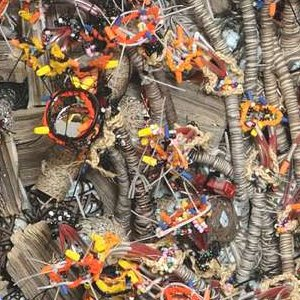
\includegraphics[width=0.33\linewidth]{./figs/regularity/22.jpg} & 
\hspace{-3mm} 
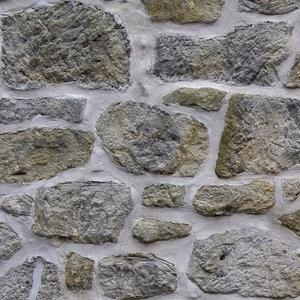
\includegraphics[width=0.33\linewidth]{./figs/regularity/13.jpg} & 
\hspace{-3mm}
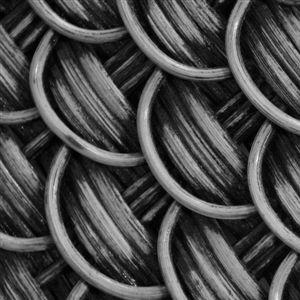
\includegraphics[width=0.33\linewidth]{./figs/regularity/90.jpg} \\ 
\scriptsize{\text{(a) 0.21}} & \scriptsize{\text{(b) 0.14}} & \scriptsize{\text{(c) 0.12}}  \\
\hspace{-1.5mm}
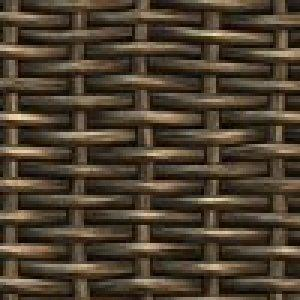
\includegraphics[width=0.33\linewidth]{./figs/regularity/57.jpg} & 
\hspace{-3mm}
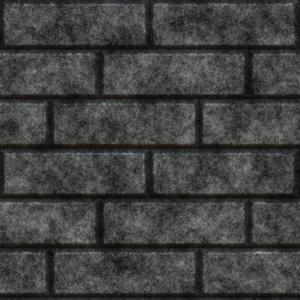
\includegraphics[width=0.33\linewidth]{./figs/regularity/28.jpg} & 
\hspace{-3mm}
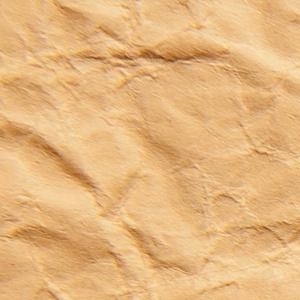
\includegraphics[width=0.33\linewidth]{./figs/regularity/44.jpg} \\ 
\scriptsize{\text{(d) 0.10}} & 
\scriptsize{\text{(e) 0.07}} & 
\scriptsize{\text{(f) 0.04}}  \\
\end{array}$}
\caption{The irregularity of texture examples captured by ensemble
  composition. Images are all of $300 \times 300$ pixels.}
  \label{fig:irreg}
\end{figure}

It is noteworthy that homogeneity, repetitiveness, and regularity
capture different properties. For instance, the texture in
Fig.~\ref{fig:homo}(b) is homogeneous, but not repetitive and not
regular. The texture in Fig.~\ref{fig:irreg}(f) is regular and
homogeneous, but not repetitive. In a nutshell, the four designed
features are not orthogonal, but are complementary.  Another thing
worth notifying is the $7$ features are not exhaustive, other features
such as entropy, coarseness, directionality, could also be relevant to
synthesizability.

\subsection{Learning methods}
We attempt to computationally quantify the synthesizability of
images. For this purpose, we train (1) a regression model on the
synthesizability scores ($1$, $0.5$ and $0$) to predict the
synthesizability of a given image, and (2) an additional classifier to
suggest the `best' ETS method to synthesize the example.  Random
Forests~\cite{randomforest} were used for both training tasks due to
its fast speed. $30$ trees were used for the Forests.

\section{Experiments}
\label{sec:experiment}
% In this section, we evaluate the task of learning synthesizability,
% and its usefulness for trimming texture examples and recognizing
% texture classes.

\subsection{Learning synthesizability}

In this section, we evaluate the contribution of all features to image
synthesizability and also investigate whether synthesizability is
learnable. In total, $10$ features were evaluated, including the $7$
single features, the combination of general features, the combination
of designed features, and the combination of all features.  $30\%$ of
data were used for training with the rest for test, and we report the
results over $5$ random training-test splits. For evaluation, we
performed two retrieval tasks and evaluate the average precision for
different recalls: (1) retrieve images with `good' scores ($>=$good);
(2) retrieve images with `good' and acceptable scores
($>=$acceptable).


\textbf{Quantitative evaluation}. Table~\ref{table:contribution} shows
the results of different features when recall is set to $1$, and
Fig.~\ref{fig:curve} shows the results of different recalls when all
features are used.  From the table, we can find that all single
features are helpful. Homogeneity performs the best among all single
features. The interesting observation is that the combination of the
designed features performs much better than the combination of the
general texture features, given it is of only $4$ dimensions. This
suggests that the designed features are more relevant to
synthesizability and serve their job very well. However, general
texture features are complementary to the designed features, given the
fact that the combination of all features yields the best
performance. Also, from the best precision ($94.5\%$ for
$>=$acceptable, and $77.0\%$ for $>=$good), we can draw the conclusion
that image synthesizability is learnable and predictable. If only a
fraction of positive examples need to be retrieved, a very high
precision is guaranteed (See Fig.~\ref{fig:curve}). This is very
useful for choosing synthesizable textures from internet images. 

\begin{figure*} [!t]
  \centering \scalebox{1}{
   $ \begin{array}{ccccc}
\hspace{-1.5mm}
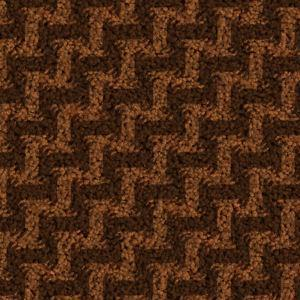
\includegraphics[width=0.13\linewidth ]{./figs/Fabric/147.jpg} & 
\hspace{-2mm} 
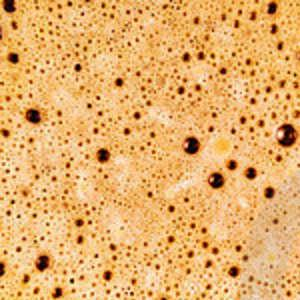
\includegraphics[width=0.13\linewidth]{./figs/fig8/bing_foam_150.jpg} & 
\hspace{-2mm}
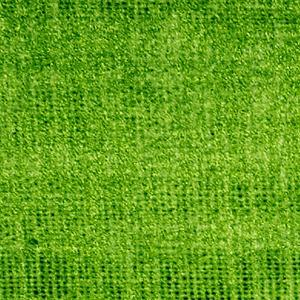
\includegraphics[width=0.13\linewidth]{./figs/Fabric/161.jpg} & 
\hspace{-2mm}
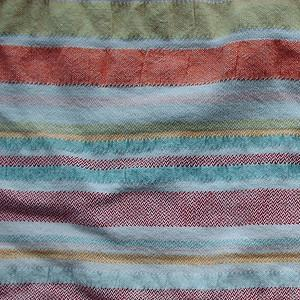
\includegraphics[width=0.13\linewidth]{./figs/Fabric/696.jpg} & 
\hspace{-2mm}
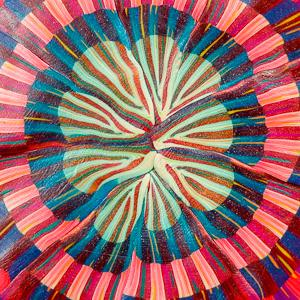
\includegraphics[width=0.13\linewidth]{./figs/Fabric/flickr_Fabric_75.jpg} \\ 

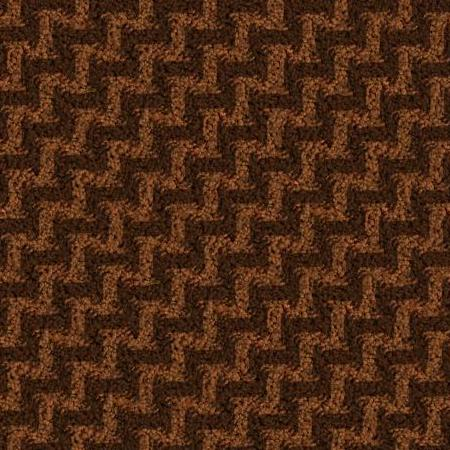
\includegraphics[width=0.195\linewidth]{./figs/Fabric/147_syn.jpg} & 
\hspace{-3mm} 
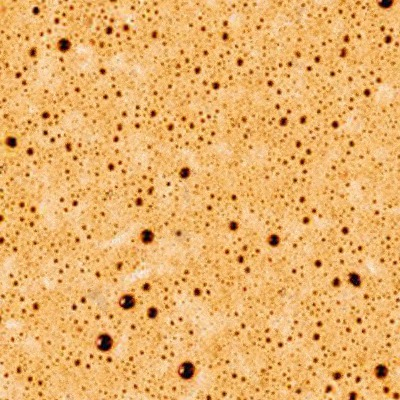
\includegraphics[width=0.195\linewidth]{./figs/fig8/bing_foam_150_m.jpg} & 
\hspace{-3mm} 
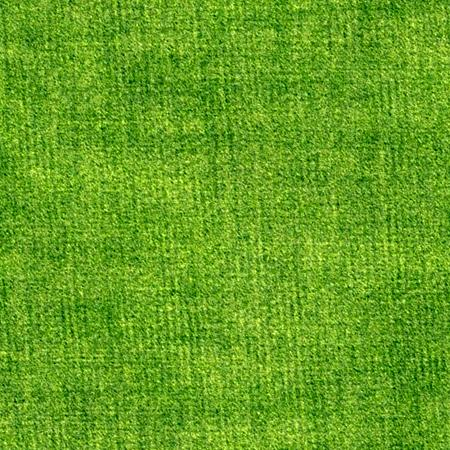
\includegraphics[width=0.195\linewidth]{./figs/Fabric/161_syn.jpg} & 
\hspace{-3mm}
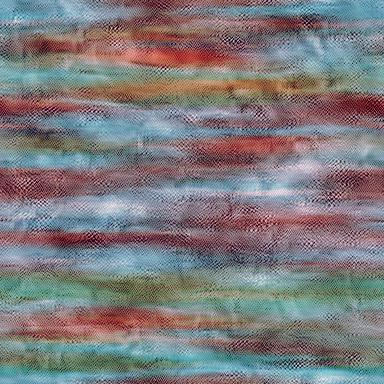
\includegraphics[width=0.195\linewidth]{./figs/Fabric/696_syn.jpg} & 
\hspace{-3mm}
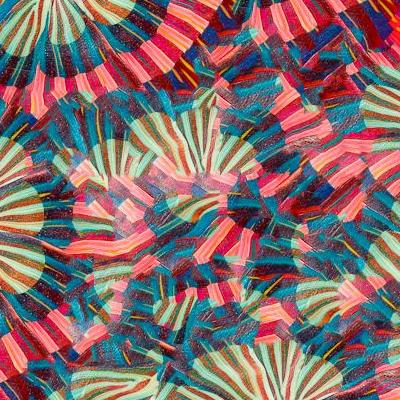
\includegraphics[width=0.195\linewidth]{./figs/Fabric/flickr_Fabric_75_q.jpg} \\ 

% \scriptsize{\text{(a) 0.98, Quilting~\cite{Efros:sig2001}}} & 
% \scriptsize{\text{(g) 0.88, MMRF~\cite{paget:tip98}}} & 
% \scriptsize{\text{(c) 0.75, Phase~\cite{random:phase}}} & 
% \scriptsize{\text{(d) 0.37, Wavelets~\cite{Portilla:2000:IJCV}}} & 
% \scriptsize{\text{(e) 0.04, Quilting~\cite{Efros:sig2001}}}  \\

\scriptsize{\text{(a) 0.98}} & 
\scriptsize{\text{(g) 0.88}} & 
\scriptsize{\text{(c) 0.75}} & 
\scriptsize{\text{(d) 0.37}} & 
\scriptsize{\text{(e) 0.04}}  \\

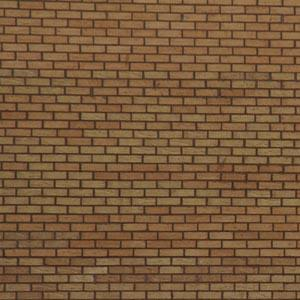
\includegraphics[width=0.13\linewidth ]{./figs/fig8/google_brick_32.jpg} & 
\hspace{-2mm}
\includegraphics[width=0.13\linewidth]{./figs/fig8/flickr_carpet_325.jpg} & 
\hspace{-2mm}
\includegraphics[width=0.13\linewidth]{./figs/fig8/bing2_rust_136.jpg} & 
\hspace{-2mm} 
\includegraphics[width=0.13\linewidth]{./figs/fig8/bing2_crowd_176.jpg} & 
\hspace{-2mm}
\includegraphics[width=0.13\linewidth]{./figs/fig8/bing2_pasta_69.jpg} \\ 

% \scriptsize{\text{(f) 0.94, Quilting~\cite{Efros:sig2001}}} & 
% \scriptsize{\text{(h) 0.79, Wavelets~\cite{Portilla:2000:IJCV}}} & 
% \scriptsize{\text{(i) 0.78, MMRF~\cite{paget:tip98}}} & 
% \scriptsize{\text{(g) 0.42, MMRF~\cite{paget:tip98}}} & 
% \scriptsize{\text{(j) 0.20, Quilting~\cite{Efros:sig2001}}}  \\
\hspace{-1.5mm}
\includegraphics[width=0.195\linewidth]{./figs/fig8/google_brick_32_q.jpg} & 
\hspace{-3mm} 
\includegraphics[width=0.195\linewidth]{./figs/fig8/flickr_carpet_325_w.jpg} & 
\hspace{-3mm}
\includegraphics[width=0.195\linewidth]{./figs/fig8/bing2_rust_136_m.jpg} & 
\hspace{-3mm} 
\includegraphics[width=0.195\linewidth]{./figs/fig8/bing2_crowd_176_q.jpg} & 
\hspace{-3mm}
\includegraphics[width=0.195\linewidth]{./figs/fig8/bing2_pasta_69_q.jpg} \\ 

\scriptsize{\text{(f) 0.94}} & 
\scriptsize{\text{(h) 0.79}} & 
\scriptsize{\text{(i) 0.78}} & 
\scriptsize{\text{(g) 0.42}} & 
\scriptsize{\text{(j) 0.20}}  \\

\end{array}$ }
\caption{The synthesizability scores of texture examples and the synthesized textures by the suggested
  synthesis method.}
  \label{fig:scoring1}
\end{figure*}


\begin{table*} [tb] \scriptsize
$\begin{array}{ccccccccccc}

\begin{tabular}{c}
\multicolumn{1}{c}{Features} \\ \hline 
$>=$Acceptable  \\\hline
$>=$Good \\ \hline
\end{tabular}


\begin{tabular}{c}
\multicolumn{1}{c}{LBP} \\ \hline 
88.4\%  \\\hline
58.3\% \\ \hline
\end{tabular}

\begin{tabular}{c}
\multicolumn{1}{c}{SFilter} \\ \hline 
77.0\%  \\ \hline
37.9\%  \\ \hline
\end{tabular}


\begin{tabular}{c}
\multicolumn{1}{c}{GIST} \\ \hline 
84.3\% \\\hline
53.1\%  \\\hline
\end{tabular}

\begin{tabular}{c}
\multicolumn{1}{c}{Textureness}  \\ \hline 
77.2\%  \\ \hline
38.5\%  \\ \hline
\end{tabular}

\begin{tabular}{c}
\multicolumn{1}{c}{Homogeneity} \\ \hline 
89.1\%  \\ \hline
64.0\%  \\ \hline
\end{tabular}

\begin{tabular}{c}
\multicolumn{1}{c}{Repetitiveness} \\ \hline 
82.2\%  \\ \hline
45.6\%  \\ \hline
\end{tabular}

\begin{tabular}{c}
\multicolumn{1}{c}{Irregularity} \\ \hline 
76.4\%  \\ \hline
39.1\%  \\ \hline
\end{tabular}

\begin{tabular}{c}
\multicolumn{1}{c}{General} \\ \hline 
88.9\%  \\ \hline
61.0\%  \\ \hline
\end{tabular}

\begin{tabular}{c}
\multicolumn{1}{c}{Designed} \\ \hline 
93.3\%  \\ \hline
74.4\%  \\ \hline
\end{tabular}

\begin{tabular}{c}
\multicolumn{1}{c}{All} \\ \hline 
94.5\%  \\ \hline
77.0\%  \\ \hline
\end{tabular}
\end{array} $
\vspace{1mm}
\centering 
\caption{The average precision of synthesizability prediction with all features (combinations), when recall is 1. 
} \label{table:contribution}
\end{table*}


\textbf{Qualitative evaluation}. Fig.~\ref{fig:synlity} and
Fig.~\ref{fig:scoring1} show examples with the synthesizability
predicted. As we can see from the figures, homogeneious, repetitive,
and regular texture examples obtain higher scores. The low scores are
caused by many factors, such as outliers, surface
distortions, and complex structures. In Fig.~\ref{fig:scoring1}, 
synthesized images by the suggested method are also shown. It is
interesting to see that the quality of the synthesized images are
largely consistent with the synthesizability score predicted. This
property is crucial because we now are able to fill the gap between
example-based texture synthesis and image retrieval (for an abundance
of textures) by filtering out the unsynthesizable retrieved images and
suggesting the `right' synthesis method for the images, thus providing
the possiblity for large-scale applications.


\textbf{Failures}. Of couse, the method fails sometime. The typical
false positives (assigning high score for unsynthesizable images) are
images with fine, global, but irregular structures, \eg crumpled paper
and fabric, wood with year rings, or foliage nerves. The reason is
that the features we used were not designed to capture these subtle,
but semantically crucial information. The typical false negatives (low
score for synthesizable images) are some very heterogeneous textures
such as rusts and clouds. This is because the space of valid textures
for these classes are very large so that synthesized textures are very
easy to fall inside the space, regardless of the fact that the examples
are very heterogeneous and irregular. See Fig.~\ref{fig:failure} for
examples. 

\textbf{Synthesizability with scales} Textures in an image can be
perceived at different scales of resolution. Thus, it is interesting
to see how scales of textures affects their
synthesizability. Fig.~\ref{fig:scale} shows an example, where three
scales of the same texture are used as the examples for
synthesizability prediction. As we can see that synthesizability score
drops with the resolution (as long as the main texture have not
switched) as more structures/objects appears. This is in keeping with
human intuition.



\begin{figure} 
 \centering
\includegraphics[width=0.8\linewidth]{./figs/AP_curve_all.pdf} \\ 
\caption{The average precision of synthesizability prediction for different recalls, when all features are used. }
  \label{fig:curve}
\end{figure}

\begin{figure} 
  \centering
   $ \begin{array}{cccc}

\hspace{-1.5mm}
\includegraphics[width=0.2\linewidth]{./figs/failure/fp/bing2_crowd_35.jpg} & 
\hspace{-3mm}
%\multirow{2}{c|}{Head 1}
\includegraphics[width=0.3\linewidth, height=23mm]{./figs/failure/fp/bing2_crowd_35_m.jpg} & 
\hspace{-3mm}
\includegraphics[width=0.2\linewidth]{./figs/failure/fp/bing2_leaves_33.jpg} & 
\hspace{-3mm}
%\multirow{2}{c|}{Head 1}
\includegraphics[width=0.3\linewidth, height=23mm]{./figs/failure/fp/bing2_leaves_33_q.jpg} \\ 
\hspace{-1.5mm}
\scriptsize{\text{ (a) 0.68}} & 
\hspace{-3mm}
\scriptsize{\text{ (b) synthesized}  } & 
\hspace{-3mm}
\scriptsize{\text {(c) 0.67}} & 
\hspace{-3mm}
\scriptsize{\text{(d) synthesized}} \\ 

\hspace{-1.5mm}
\includegraphics[width=0.2\linewidth]{./figs/failure/fn/bing2_cloud_68.jpg} & 
\hspace{-3mm}
%\multirow{2}{c|}{Head 1}
\includegraphics[width=0.3\linewidth, height=23mm]{./figs/failure/fn/bing2_cloud_68_q.jpg} & 
\hspace{-3mm}
\includegraphics[width=0.2\linewidth]{./figs/failure/fn/bing2_rust_71.jpg} & 
\hspace{-3mm}
%\multirow{2}{c|}{Head 1}
\includegraphics[width=0.3\linewidth, height=23mm]{./figs/failure/fn/bing2_rust_71_q.jpg} \\ 
\hspace{-1.5mm}
\scriptsize{\text{ (e) 0.11}} & 
\hspace{-3mm}
\scriptsize{\text{ (f) synthesized}  } & 
\hspace{-3mm}
\scriptsize{\text {(g) 0.32}} & 
\hspace{-3mm}
\scriptsize{\text{(h) synthesized}} \\ 

\end{array}$
\caption{Failure cases: the top shows false positives and the bottom
  false negatives. Examples are of $300 \times 300$ pixels.}
  \label{fig:failure}
\end{figure}



\begin{figure} 
  \centering
   $ \begin{array}{ccc}
\hspace{-1.5mm}
\includegraphics[width=0.33\linewidth]{./figs/scale/flickr_crushed_78.jpg} & 
\hspace{-3mm}
\includegraphics[width=0.33\linewidth]{./figs/scale/flickr_crushed_79.jpg} & 
\hspace{-3mm}
\includegraphics[width=0.33\linewidth]{./figs/scale/flickr_crushed_80.jpg} \\
\scriptsize{\text{ (a) 0.15}} & 
\scriptsize{\text{ (b) 0.50}} & 
\scriptsize{\text{ (c) 0.89}} \\ 
\end{array}$
\caption{Synthesizability with scales of textures. }
  \label{fig:scale}
\end{figure}


% We also show and compare the synthesizability of different texture
% categories (the average synthesizability of all images of the
% category).  The UIUC texture dataset~\cite{UIUC:Texture}, which
% contains $25$ texture categories, each with $40$ images. Fig.~\ref{}
% shows the synthesizability of all categories (average of
% synthesizability of all texture examples in each category). From the
% figure, we find that ...

% This characterization could be further analyzed in terms of different
% texture materials, different illumination conditions, different scales
% of textures, and so on. The characterization of textures of
% Columbia-Utrecht Reflectance and Texture
% Database~\cite{columbia:texture} and Open-Surface
% dataset~\cite{open:surface} is planned as a future work. The former
% one is about different illuminations, and the latter is for real-world
% semantic textures.




\subsection{Trimming texture examples}
In this section, image synthesizability is used for trimming images to
more synthesizable parts. Given an image, the image synthesizability
of all its subimages is computed and compared. The most synthesizable
subimage is then suggested. See Fig.~\ref{fig:roi} for examples. $500$
sub-windows were randomly sampled, with the mimimum scale being of
$100 \times 100$ pixels and the maximum scale being the size of the
image. The figure suggests that our method performs well for this
task.  This ability delivers the possibility of obtaining
synthesizable texture examples from unconstrained images. See
Fig.\ref{fig:roisyn} for why it is useful.

%  A method to detect the synthesizable textures in images is very
% useful.
% This trimming shares some similarity with~\cite{dominant:texture:09}
% but is still different. They detect the
% dominant texture within an image; we are interested in detecting the
% most synthesizable parts.

\subsection{Texture recognition}
In this section, we evaluate the usefulness of synthesizability and
the $4$ designed features (synfets) for texture recognition. The UIUC
texture dataset~\cite{UIUC:Texture} was used for this task, which
contains $25$ texture categories, each with $40$ images. Linear SVMs
were used as the classifier, with $C=10$. We show the classification
accuracy of Uniform LBP~\cite{lbp:2002}, of synfets, and of the
concatenation of them. For all experiments, $12$ training images per
class were used, and the reported accuracy was computed over $10$
random training-test splits.  The result is listed in
Table~\ref{table:recognition}, which shows that synfets complement
normal texture features for texture recognition. More generally, the
self-relationships captured by our designed features also play roles
in defining texture categories.

% \subsection{Describing textures}
% We also validate the effectiveness of the four designed
% features as general texture attributes. The evaluation is based on pairwise
% comparison: given an image pair, we predict which image exhibits the
% attributes more than the other. The prediction results are compared to
% manual annotation for evaluation.  For this purpose, we labeled
% $600$ randomly chosen image pairs from the $2000$ general textures in
% terms of the comparison of the four texture
% attributes. Table~\ref{table:fet} lists the accuracy of the
% predictions.  The results show that the methods we designed for the
% four general texture attributes perform fairly well: the computed 
% comparisons correlate well with the human comparisons. We use the four
% features for synthesizability learning, but they can be used for other
% tasks as well, such as texture indexing. 



\begin{figure*} [!t]
  \centering
   $ \begin{array}{cccc}
\hspace{-1.5mm}
\includegraphics[width=0.24\linewidth, height=35mm]{./figs/2/2.jpg} & 
\hspace{-3mm}
\includegraphics[width=0.24\linewidth, height=35mm]{./figs/2/3.jpg} & 
\hspace{-3mm}
\includegraphics[width=0.24\linewidth, height=35mm]{./figs/2/22_1.jpg} & 
\hspace{-3mm}
\includegraphics[width=0.24\linewidth, height=35mm]{./figs/2/22_3.jpg} \\
\scriptsize{\text{ (a) RS:\textcolor{red}{0.92} \hspace{1mm} IS:0.40}} & 
\scriptsize{\text{ (b) RS:\textcolor{red}{0.67}, \hspace{1mm} IS:0.50}}  &
\scriptsize{\text{ (c) RS:\textcolor{red}{0.63} \hspace{1mm} IS:0.42}} & 
\scriptsize{\text{ (d) RS:\textcolor{red}{0.74} \hspace{1mm} IS:0.43}} \\ 
\end{array}$
\caption{The most synthesizable region detected.  Synthesizability of
  detected regions (RS) and the whole images (IS) are shown. }
  \label{fig:roi}
\end{figure*}


\begin{figure} 
  \centering
   $ \begin{array}{ccc}
\hspace{-1.5mm}
\includegraphics[width=0.30\linewidth]{./figs/roi/roi_2.jpg} & 
\hspace{-3.5mm}
\includegraphics[width=0.34\linewidth, height=22mm]{./figs/roi/2_syn.jpg} & 
\hspace{-3.5mm}
\includegraphics[width=0.34\linewidth, height=22mm]{./figs/roi/2_1_syn.jpg} \\

\hspace{-1.5mm}
\scriptsize{ \text{(a) IS:0.05 \hspace{1mm} RS:\textcolor{red}{0.58}}} & 
\hspace{-3.5mm}
\scriptsize{\text{(b) Synthesized out of image}} & 
\hspace{-3.5mm}
\scriptsize{\text{ (c) Synthesized out of region}} \\
 
\hspace{-1.5mm}
\includegraphics[width=0.30\linewidth]{./figs/roi/roi_1.jpg} & 
\hspace{-3.5mm}
\includegraphics[width=0.34\linewidth, height=22mm]{./figs/roi/1_syn.jpg} & 
\hspace{-3.5mm}
\includegraphics[width=0.34\linewidth, height=22mm]{./figs/roi/1_1_syn.jpg} \\
\hspace{-1.5mm}
\scriptsize{ \text{ (d) IS:0.18 \hspace{1mm} RS:\textcolor{red}{0.50}}} & 
\hspace{-3.5mm}
\scriptsize{\text{ (e) Synthesized out of image}} & 
\hspace{-3.5mm}
\scriptsize{\text{ (f) Synthesized out of region}} \\ 

\end{array}$
\caption{Synthesizability of the image (IS) and the detected region
  (RS), and the synthesized textures from the image and region. }
  \label{fig:roisyn}
\end{figure}

\begin{table}[tb] \footnotesize 
$\begin{array}{ccccc}
\begin{tabular}{c|}
\multicolumn{1}{c|}{Feature} \\ \hline 
Accuracy (\%) \\ 
\end{tabular}

\begin{tabular}{c}
\multicolumn{1}{c}{\scriptsize{LBP}} \\ \hline 
68.1 (2.1)  \\ 
\end{tabular}

\begin{tabular}{c}
\multicolumn{1}{c}{\scriptsize{Synfets}} \\ \hline
31.1 (1.6)   \\ 
\end{tabular}

\begin{tabular}{c}
\multicolumn{1}{c}{\scriptsize{LBP + Synfets}} \\ \hline 
69.7(1.6)   \\ 
\end{tabular}
\end{array} $
\vspace{1mm}
\centering 
\caption{Classification accuracy on Texture-25 dataset.} \label{table:recognition}
\end{table}




% \begin{table} \footnotesize 
% $\begin{array}{ccccc}
% \begin{tabular}{c|c}
% \multicolumn{1}{c|}{Features} \\ \hline
% Accuracy \\  
% \end{tabular}

% \begin{tabular}{c}
% \multicolumn{1}{c}{\scriptsize{Textureness}} \\ \hline 
% 89.1\%  \\
% \end{tabular}

% \begin{tabular}{c}
% \multicolumn{1}{c}{\scriptsize{Homogeneity}} \\ \hline 
% 79.4\%  \\ 
% \end{tabular}

% \begin{tabular}{c}
% \multicolumn{1}{c}{\scriptsize{Repetitiveness}} \\ \hline 
% 82.5\%  \\ 
% \end{tabular}

% \begin{tabular}{c}
% \multicolumn{1}{c}{\scriptsize{Regularity}} \\ \hline 
% 75.2\%  \\ 
% \end{tabular}
% \end{array} $
% \vspace{1mm}
% \centering 
% \caption{Accuracy of the four designed texture features. 
% } \label{table:fet}
% \end{table}


\section{Conclusions}
\label{sec:conclusion}
The paper proposed synthesizability as a novel texture property and
developed a computational predictor for it. We constructed a fairly
large dataset and calibrated it according to synthesizability. A set
of texture features have been proposed and, in some cases, designed
for the learning, such as textureness, homogeneity, repetitiveness,
irregularit. Their usefulness has been verified for multiple
tasks. Extensive experiments show that image synthesizability can be
learned and predicted computationally. It can be used to find good
texture examples for synthesis, to detect good textures from
unconstrained images for synthesis, and to choose an appropriate
method to do so. It also is a useful feature for texture recognition.


\vspace{1.5mm}
\noindent
\textbf{Reproductivity.} The Code and Data are available at the project page:\url{www.vision.ee.ethz.ch/~daid/synthesizability}.

\vspace{1.5mm}
\noindent
\textbf{Acknowledgements.} The work is supported by the ERC Advanced Grant VarCity and 
the ETH-Singapore project Future Cities.


{\footnotesize
\bibliographystyle{ieee}
\bibliography{egbib}
}

\end{document}
